\chapter{Implementation} \label{chap:Implementation}

%intro words

This chapter then presents the concepts underlying Distributed Abstract Data
Types (DADTs), a short description of existing DADT prototype
\cite{migliavacca_DADT:2006}, and an outline of the limitations of the current
prototype.

, and how LNs can be used to eliminate the
limitations inherent in the DADT prototype

The chapter then concludes 
with a description of the simulation environment \cite{barr_JIST:2005}, \cite{barr_SWANS} underlying the 
implementation, and the hardware platform - Sun Small Programable Object
Technology (SPOT) \cite{simon_squawk:2006} - used during the course of this work
to experimentally validate the simulated implementation in a
real-world environment. 


\section{Contribution}

\cite{migliavacca_DADT:2006} presented a prototype that enabled the use of DADTs
to facilitate distributed application programming. While this approach is
clearly applicable to WSNs, the prototype itself did not support WSN
abstractions, and there were several limitations to it:

\begin{itemize}
  \item The lack of a routing mechanism.
  \item Limitations in portability to real WSN nodes.
\end{itemize}

This work makes the following contributions:

\begin{itemize}
  \item Extension of the DADT prototype for use in WSNs by extending it to run
  on simulators as well as devices in a real-world environment.
  \item Interfacing the LN mechanism presented in \cite{mottola_LNAbstraction}
  to enable abstracted communication between groups of nodes in the WSN defined
  by DADTs.
  \item  Verification of the utility of DADT abstractions in the WSN application
  layer.
\end{itemize}

\section{The DADT/LN Architecture}

% FILL THIS IN LATER.
\subsection{Overview}
\begin{figure}
\centering
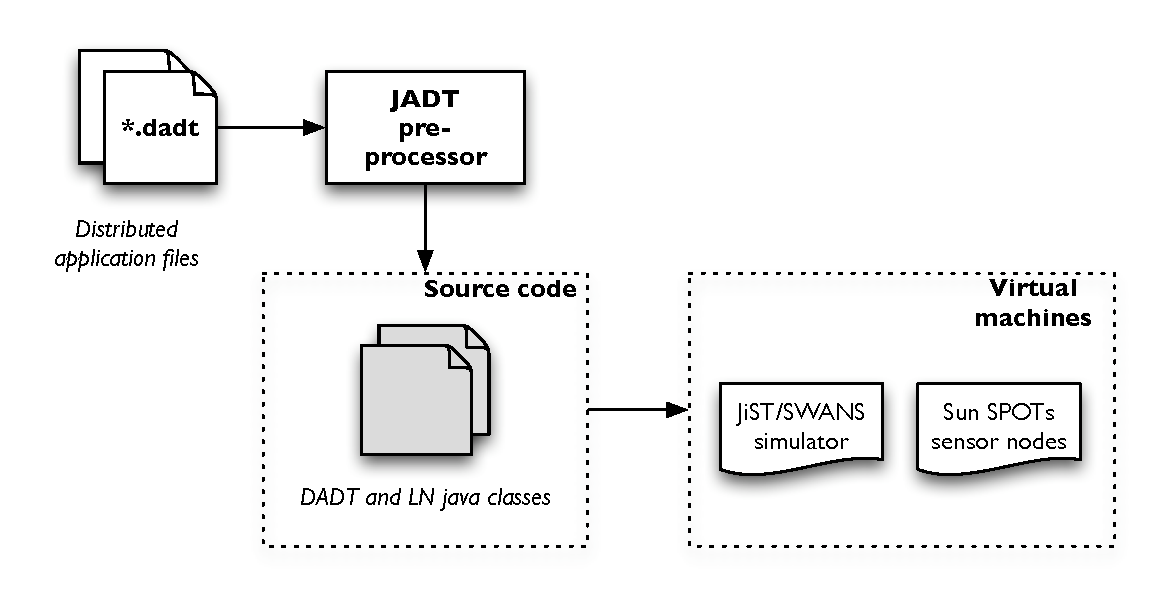
\includegraphics[width=\textwidth]{img/DADTLN_architecture.eps} 
\caption[DADT/LN application workflow]{Workflow for development of an application that uses
the DADT/LN prototype}
\label{Fig:DADTLN_architecture}
\end{figure} 
The overview of the workflow involved in using DADTs to enable WSN application
programming is as shown in Figure \ref{Fig:DADTLN_architecture}. The user writes
application layer code for the WSN using a DADT language in a series of
\emph{.dadt} files. A preprocessor is used to convert the code written by the
application programmer into Java code that interfaces with the DADT
infrastructure (extended from the prototype presented in
\cite{migliavacca_DADT:2006}). In order to facilitate routing to LNs defined by
the use of DADT views, the DADT infrastructure is interfaced with the a
previously developed implementation of LNs. 

The application (including the implementation of layers lower in the protocol
stack) is then loaded on to either:
\begin{itemize}
\item the JiST/SWANS simulator \cite{barr_JIST:2005, barr_SWANS}. See Section \ref{sec:jistswans} for details on the implementation of
the aforementioned simulator
\item a collection of Sun SPOT wireless sensor devices \cite{simon_squawk:2006}
(see Section \ref{sec:sunspots}) to execute the application on real sensor nodes.
\end{itemize}

\subsection{Explanation of terms used}

\begin{figure}
\centering
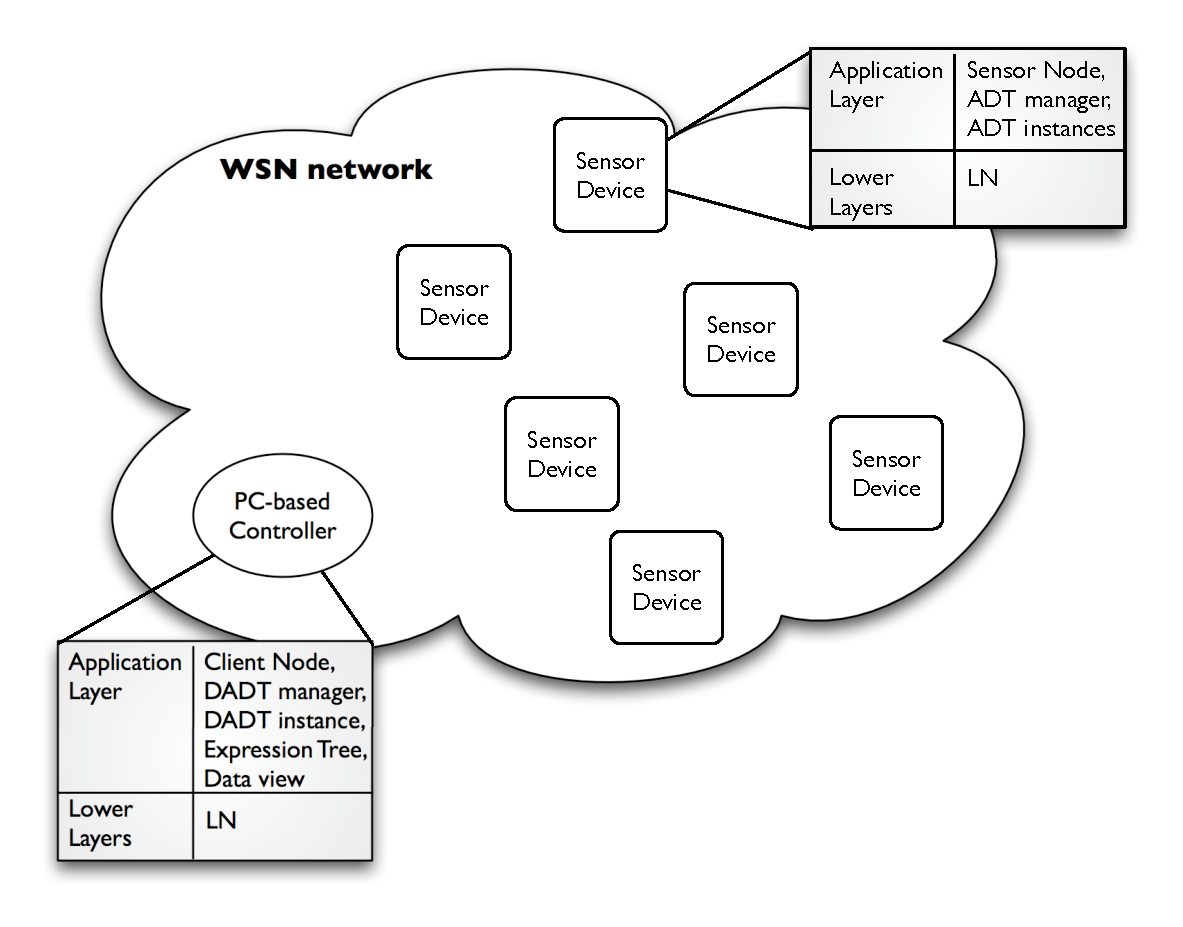
\includegraphics[scale=0.55]{img/DADTLN_glossary.eps} 
\caption[WSN in DADT/LN prototype]{Schematic Representation of the WSN as abstracted in the DADT/LN prototype}
\label{Fig:DADTLN_glossary}
\end{figure} 

This section explains the terms used in the DADT/LN prototype developed as part
of this work. The WSN network in this prototype consists of two types of
devices as shown in Figure \ref{Fig:DADTLN_glossary}: 
\begin{itemize}
  \item \emph{Controller:} Typically PC-based, this node contains in the
  application layer the client node, the expression tree, the DADT instance, the
  DADT manager; the LN
  implementation is used in the network layer. The user's application code resides on
  the controller node.
  \item \emph{Sensor Device:} This is a sensor device such as a Sun SPOT, and
  holds the following entities:
  \begin{itemize}
    \item \emph{Application Layer:} It includes a Sensor Node that in turn
    consists of multiple sensor ADT instances, and an ADT manager.
    \item \emph{Network Layer:} The LN implementation is used.
  \end{itemize}
\end{itemize}

\subsection{Execution Details}

This section attempts to explain the operation of the DADT/LN prototype
developed as part of this work by considering the sequence of method calls made
during execution. The operation of the simulation platform as well as the
nodes itself is abstracted from the explanations that follow, as is the actual
\emph{.dadt} syntax used by the application programmer himself to trigger these
operations. 

\subsubsection{The DADT/LN prototype on the Controller}

Figure \ref{Fig:SeqDiagram_Sensornode} presents the operation of the DADT/LN
prototype on the controller (which is typically PC-based). As shown in the figure, the implementation running on each sensor node 
consists of the following entities:

\begin{itemize}
  \item \emph{Client Node:} A Client Node is an abstraction that consists of a
  DADT instance. The application programmer's requests to the network are issued
  by the Client Node.
  \item \emph{DADT Instance:} A DADT Instance is explained in Section
  \ref{subsubsec:dadtspecandinst}, and allows for collective access to multiple
  ADT instances.
  \item \emph{Expression Tree:} An expression tree is a specific construct that is to
  build a hierarchical data view.
  \item \emph{DADT Manager:} The DADT Manager provides the interface between the
  Client Node and the network, and passes request messages from the Client Node
  to the lower layers of the protocol stack.
  \item \emph{Data View:} Data views are explained in Section
  \ref{subsubsec:views}, and is a mechanism for partitioning the collection of
  ADT instances bound to a particular DADT type.
\end{itemize}

The instantiation of a DADT type by the application programmer's
code\footnote{This is written in the DADT specification language.} causes the
following actions to take place at the Controller:
\begin{itemize}
  \item The Client Node creates an instance of the DADT type that is used to perform
collective operations on the network.  
\item A new expression tree is created to provide a hierarchical representation
of the application programmer's definition of a data view.
\item The DADT instance creates an instance of the DADT manager.
\end{itemize}

When the application programmer's code requests the execution of a distributed operation
on the WSN, the following actions take place:

\begin{itemize}
  \item The Client Node forwards the request to the DADT instance. The DADT instance:
  \begin{itemize} 
    \item creates a Data
  view using the expression tree (see above),
  \item subsequently uses the DADT 
  manager to construct LN predicates from the expression, 
  \item sends a
  request message to the network using the DADT manager, and
  \item sleeps until the result of the computation is
  received from the network layer \emph{(N.B.: The DADT instance is implemented as a
  separate thread)}.
  \end{itemize}
  \item When the result of the distributed computation is received, the Client Node is notified. 
 The Client Node then executes
  the appropriate function on the DADT instance to collect and process the
  readings. The DADT instance returns the processed readings to the Client Node.
\end{itemize}


\subsubsection{The DADT/LN prototype on the sensor device} \label{subsubsec:DADTLNSensorDevice}

Figure \ref{Fig:SeqDiagram_Sensornode} presents the operation of the DADT/LN
prototype on the sensor device (which may be either simulated or a real
device). As shown in the figure, the implementation running on each sensor node 
consists of the following entities:

\begin{itemize}
  \item \emph{Sensor Node:} A sensor node is an abstraction that consists of a
  list of sensors. This follows from the example used to illustrate the concept
  of ADTs in Section \ref{sec:DADT}\footnote{The term \emph{device} is used to
  refer to the physical sensor node entity, while the term \emph{sensor node}
  refers to the application layer abstraction of all of the sensors within the
  device. This abstraction resides on the device.}
  \item \emph{Sensor ADT instance:} This is an ADT instance for a given sensor
  on the sensor node upon which the prototype executes. 
  \item \emph{ADT Manager:} The ADT manager provides the interface between the
  sensor node and the network, thereby abstracting sensor ADT instances from
  queries issued by the DADT instance at the (PC-based) controller.
\end{itemize}

Sensor ADT instance intialisation is performed possibly
multiple times
on a given Sensor Node, as a node might consist of multiple sesnsors. Following
this, the sensor ADT instances are bound to a particular DADT type by calling
the ADT manager\footnote{The ADT manager is assumed in our
current implementation to be aware of all DADT types defined in the WSN.}.

When the lower layer (which runs the LN algorithm) delivers a message to the
Sensor Node, the ADT Manager is used to processed the request message.The
request message contains a DADT Data view (see Section \ref{subsubsec:views})
which is used to filter from the sensor ADT instances on the given Sensor node
those that fit into the Data view. % DOUBLE PROCESSING. YOU KNOW. I SUGGEST GET% RID OF IT.

\emph{N.B.: If the request message is received in the application layer, then at least
one of the sensor ADT instances in the Sensor Node fits into the dataview, as
the data view is expressed in the form of an LN predicate. This minimises the
number of messages received at the application layer. However, since a given
Sensor Node may contain several sensor ADT instances, the ADT instances have to
be filtered.}

The request message also contains a description of the DADT action to be
performed on-device (see Section
\ref{subsubsec:OperatorsAndActions}). The ADT manager calls the action for each
sensor ADT instance that fits into the DADT Data view. 

If the application layer requires that a reply be sent, the LN implementation in
the lower layer of the protocol stack is used as it can be seen on the bottom
right section of Figure \ref{Fig:SeqDiagram_Sensornode}.

\begin{sidewaysfigure}[htbp]
\centering
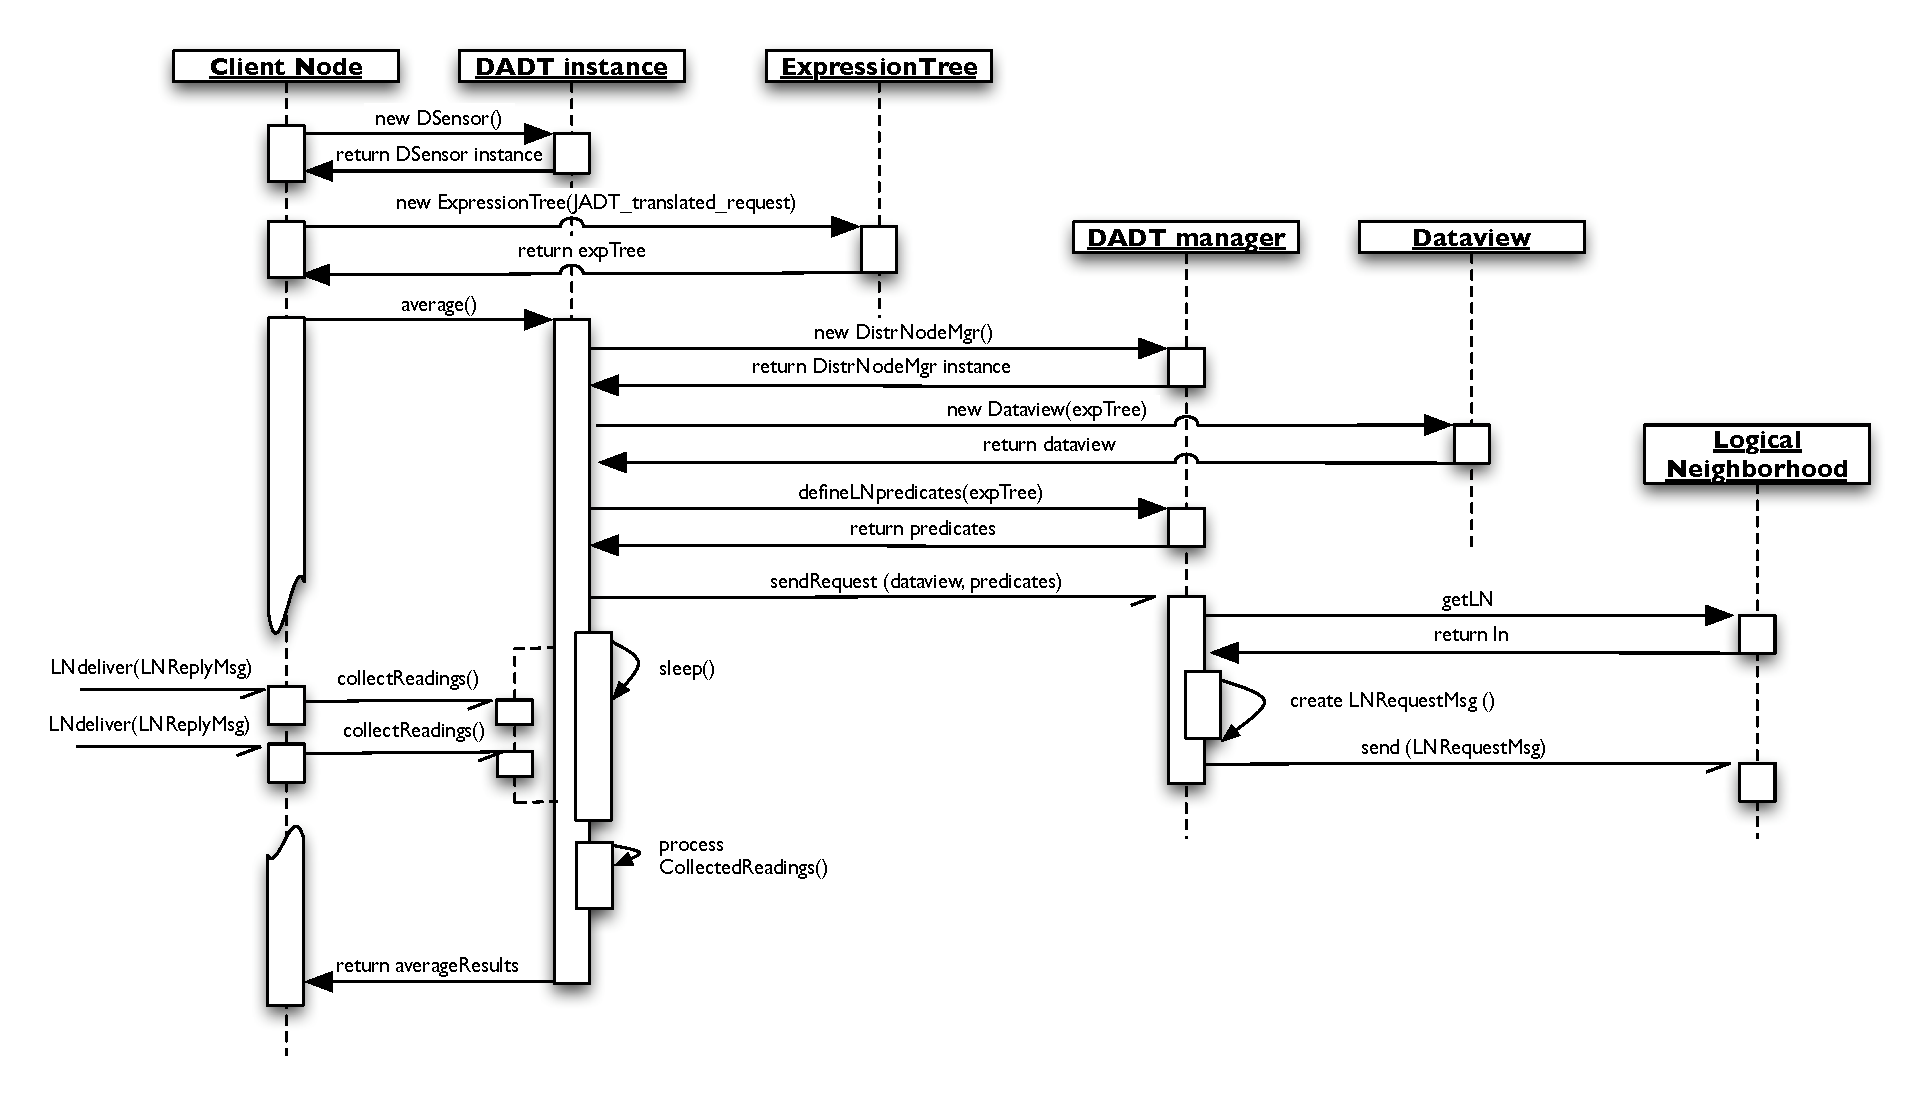
\includegraphics[width=\textwidth]{img/SeqDiagram_PCnode.eps}
\caption[Operation of the DADT/LN prototype on Controller]{Operation of the DADT/LN prototype on Controller}
\label{Fig:SeqDiagram_PCnode}
\end{sidewaysfigure}


\begin{sidewaysfigure}[htbp]
\centering
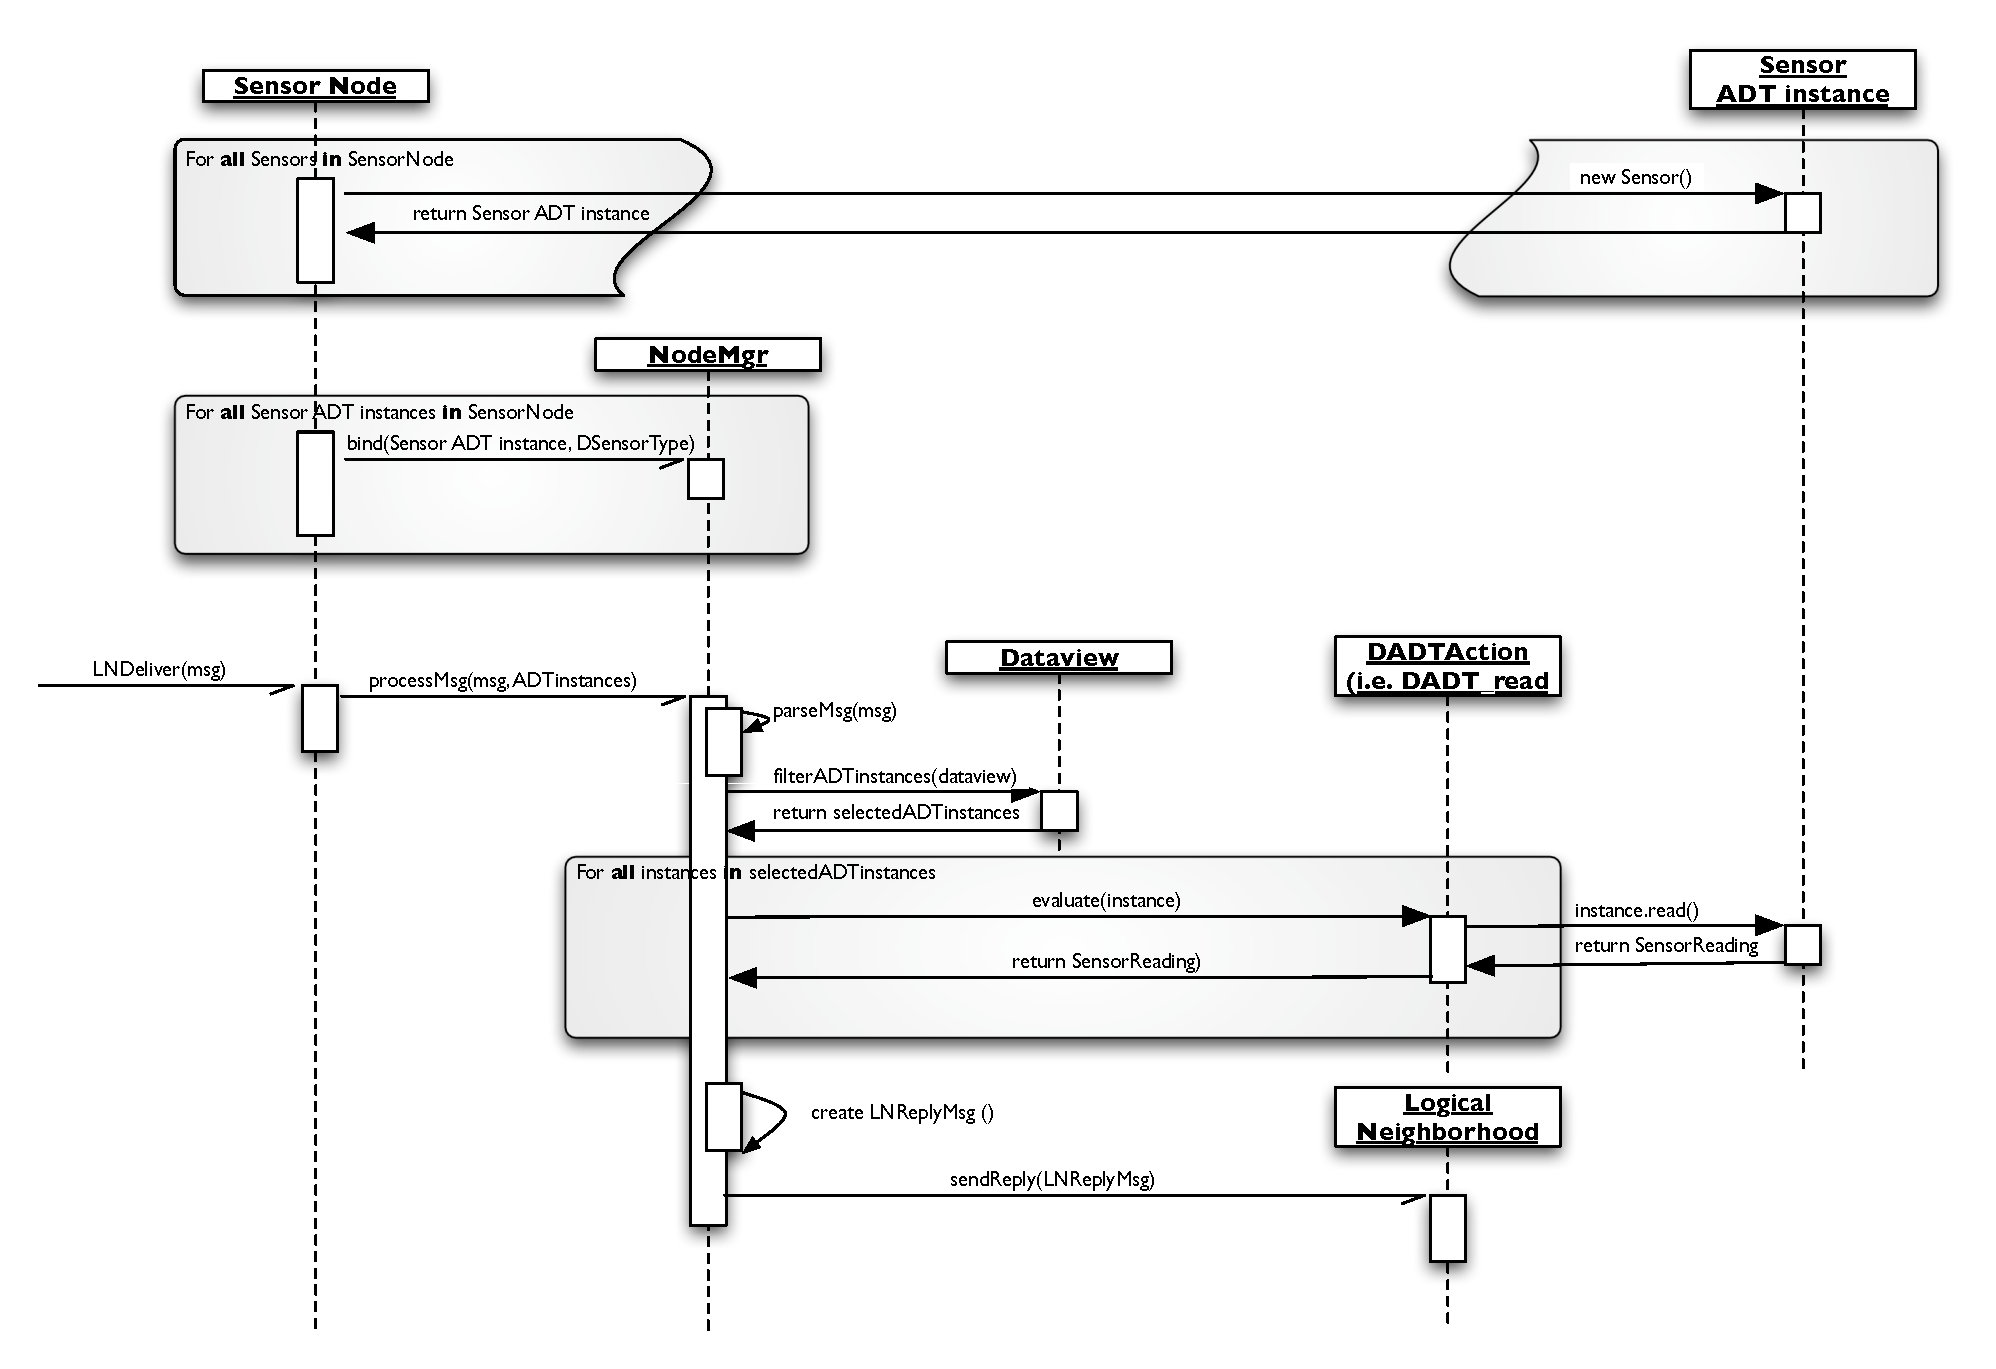
\includegraphics[width=\textwidth]{img/SeqDiagram_Sensornode.eps}
\caption[Operation of the DADT/LN prototype on sensor device]{Operation of the DADT/LN prototype on sensor device}
\label{Fig:SeqDiagram_PCnode}
\end{sidewaysfigure}

\section{The DADT/LN prototype in the simulated environment}
\subsection {JiST/SWANS} \label{sec:jistswans}

As the simulator used in this work is a discrete event simulator, this section 
begins with a short description of discrete event simulators. 
This is followed by a discussion on a particular discrete event simulator
called JiST, and the SWANS network simulator built on top of JiST.

\subsubsection{Discrete Event Simulator}

A discrete event simulator allows for the simulated execution of a process (that
may be either deterministic or stochastic), and consists of the following
components \cite{Shankar_DiscreteEventSim}:

\begin{itemize}
  \item \emph{Simulation variables:} These variables keep track of simulation 
  time, the list of events to be simulated, the (evolving) system state, and 
  performance indicators.
  \item \emph{Event handler:} The event handler schedules events for execution 
  at specific points in simulation time (and unschedules them if necessary), 
  and additionally updates the state variables and performance indicators.
\end{itemize}
 
\subsubsection{Java In Simulation Time (JiST)} \label{subsec:jist}

JiST \cite{barr_JIST:2005} is a discrete event simulator that is 
efficient (compared to existing simulation systems), 
transparent (simulations are automatically translated to run with the 
simulation time semantics), and standard (simulations use a
conventional programming language, i.e., Java).

JiST simulation code is written in Java, and converted to run over the JiST 
simulation kernel using a bytecode-level rewriter\footnote{N.B.: The bytecode 
rewriter and the simulation kernel are both written in Java},  as it can be
seen in Figure \ref{Fig:JiST_architecture}.

The execution of a JiST program can be understood by considering example as
shown in Listing \ref{listing:JiSTExample}

\begin{lstlisting}[frame=trbl, basewidth={0.55em, 0.6em}, captionpos=b, 
basicstyle=\ttfamily\footnotesize, breaklines, caption = Example JiST program (reproduced from \cite{barr_JIST:2005}, label = listing:JiSTExample]  
import jist.runtime.JistAPI;  
class hello implements JistAPI.Entity { 
  public static void main(String[] args) { 
    System.out.println("Simulation start"); 
    hello h = new hello(); 
    h.myEvent(); 
  } 
  public void myEvent() { 
    JistAPI.sleep(1); 
    myEvent(); 
    System.out.println("hello world, " + JistAPI.getTime()); 
  }} 
\end{lstlisting}

\begin{figure}
\centering
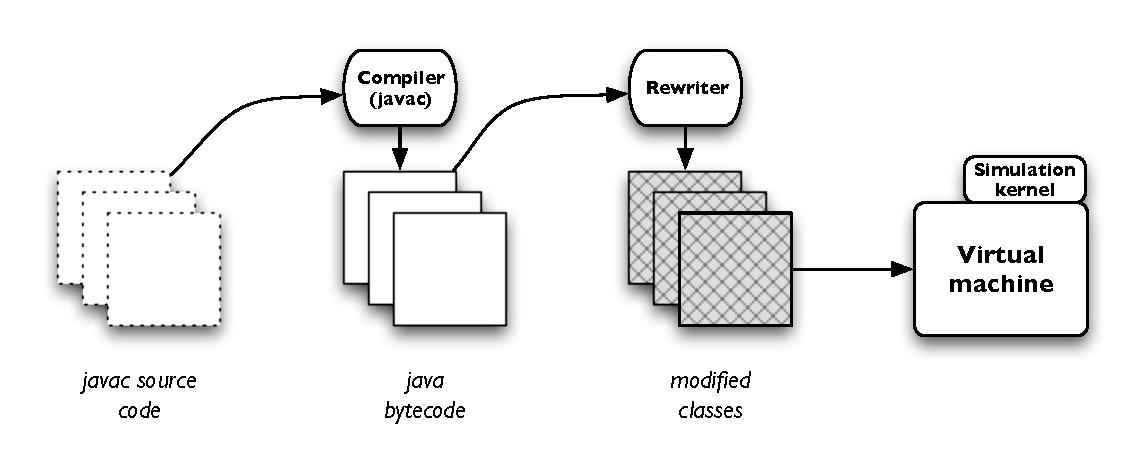
\includegraphics[width=\textwidth]{img/JiST_architecture.eps} 
\caption[The JiST System Architecture]{The JiST system architecture (reproduced from
\cite{barr_JIST:2005})}
\label{Fig:JiST_architecture}
\end{figure}  
 
This program is then compiled and executed in the JiST simulation
kernel, using the following commands:

  
\begin{lstlisting}[frame=trbl, basewidth={0.55em, 0.6em}, captionpos=b, 
basicstyle=\ttfamily\footnotesize, breaklines, caption = Execution of the
program in the JiST, label = listing:JiST ]  
javac hello.java
java jist.runtime.Main hello
\end{lstlisting}


The simulation kernel is loaded upon execution of this command. This kernel
installs into the JVM a class loader that performs the rewrite of the bytecode.
The JistAPI functions used in the example code are used to perform the
code transformations. The method call to myEvent is now scheduled and executed
by the simulator in simulation time. Simulation time differs from ``actual''
time in that the advancement of actual time is independent of application
execution. 
 
\subsubsection{Scalable Wireless Ad hoc Network Simulator (SWANS)}
SWANS is a wireless network simulator developed in order to provide efficient
and scalable simulations without compromising on simulation detail \cite{barr_SWANS},
and is built upon the JiST discrete event simulator described in Section \ref{subsec:jist}. 
It is organised a a collection of independent, relatively simple, event driven
components that are encapsulated as JiST entities. 
  
SWANS has the following capabilities \cite{barr_SWANS}:

\begin{itemize}
\item The use of
interchangeable components enables the construction of a protocol stack for the
network, and facilitates parallelism, and execution in a distributed environment.
\item Can execute unmodified Java network applications on the
simulated network (in simulation time), by virtue of its being built over
JiST.Using a harness, the aforementioned Java code is automatically rewritten to
run on the simulated network.  
\end{itemize}
   
The SWANS architecture may be seen in Figure \ref{Fig:SWANS_architecture}. 

\begin{figure}[ht]
\centering
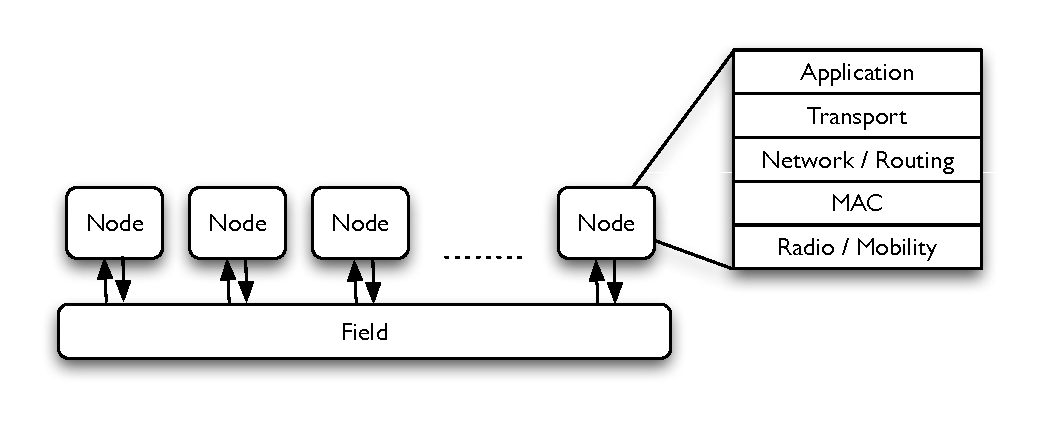
\includegraphics[width=\textwidth]{img/SWANS_architecture.eps} 
\caption[SWANS architecture]{SWANS architecture}
\label{Fig:SWANS_architecture}
\end{figure} 


\subsection{Simulation using JiST/SWANS}

The DADT/LN prototype was tested on the SWANS WSN simulator, that is buit upon
the JiST discrete event simulator (see Section \ref{subsec:jist}). 

The DADT/LN prototype code is wrapped in the JiST API, and is loaded on to a
simulated node. As described in the previous section, there are two kinds of
nodes in the DADT/LN prototype:

\begin{itemize}
  \item \emph{Controller Node}, that holds the distributed application, and the
  framework to manage the same.
  \item \emph{Sensor Device}, that holds the individual ADT instances. 
\end{itemize}

The Controller Node was implemented as a separate node on the JiST/SWANS
simulator, and was assumed not to be PC-based for the purposes of simulation.
The Sensor Device implementation (see Section
\ref{subsubsec:DADTLNSensorDevice}) was loaded on to all but one of the nodes in
the simulator.

The simulation was run on networks of upto 50 nodes to empirically verify the
robustness of the work done as part of this thesis.

\section{The DADT/LN prototype on Sun SPOTs}

For further experimental validation of the implementation produced as part of 
this thesis,
the DADT/LN prototype was deployed on Sun SPOTs \cite{simon_squawk:2006}. 

The
Controller application was executed as a host application on the host machine (a
PC), while the other Sun SPOTs ran the Sensor Device implementation as on-SPOT
applications (see Section \ref{subsec:sunspotapps} for a description of host and on-SPOT
applications).

\section{Challenges}


\section{Future Work}

This section presents a list of possible extensions to the work implemented as
part of this thesis. These include:

\begin{itemize}
  \item \emph{Support for DADT selection operators:} The current prototype
  supports the selection of all ADT instances that match a defined DADT Data
  view, but does not enable the selection of a subset of the aforementioned
  collection of ADT instances. This arises due to limitations in the current LN implementation.
  \item \emph{Extending support for Space DADTs:} Currently, the prototype does
  not use the notion of space. Therefore, a possible avenue for future work
  could include the implementation of Space DADTs, and the definition of Space
  views that are analogous to Data views.
  \item \emph{Extending the prototype for networks of heterogenous nodes:}
  The current prototype, by virtue of it being implemented in Java, cannot be
  used on a wide variety of different nodes. 
\end{itemize}

\section{Evaluation}

The performance of the DADT/LN prototype was evaluated using the following
metrics: 
\begin{itemize}
  \item Packet processing workload on the application layer.
  \item Ease of implementation. 
\end{itemize}

The first metric was used to compare the performance of the DADT/LN prototype
against that of the original DADT prototype used as the basis for this work
\cite{migliavacca_DADT:2006}. In the original DADT prototype, a request message
was replied to or discarded on the basis of an expression tree evaluation in the
application layer. In the implementation presented in this work, the integration
with the LN approach results in unsuitable request messages being discarded on
the basis of predicate evaluation in the network layer. 


A series of simulations were run using the JiST/SWANS simulations to determine
the number of request messages discarded at the network layer and the number
passed on to the application layer by the LN predicate matching algorithm. The
sum provides the total number of packets processed in the application layer of
the original DADT prototype.

It was found that the number of messages processed in the application layer was
lower in the implementation produced as part of this work.

%HOW CAN WE SAY LN PREDICATE EVAL IS MORE EFFICIENT THAN EXPRESSION TREE?

The second metric used the number of lines of code required to implement a
simple distributed averaging application. While not an ideal metric, it
quantifies the difference in the order of magnitude of coding effort required on
the part of the application programmer to produce WSN applications with and
without the use of programming abstractions. To this end, a simple WSN
application was written on the Sun SPOTs to calculate the distributed average.

The difference in the number of lines was *SDDS*.

\section{Analysis of Results}

%HERE MORE BLAH BLAH